\documentclass{article}
\usepackage[utf8]{inputenc}
\usepackage{float}
\usepackage{graphicx}   
\title{FEMM - Homework}
\author{Steinarr Hrafn Höskuldsson}
\date{January 2023}
\usepackage{listings}
\usepackage{color} %red, green, blue, yellow, cyan, magenta, black, white
\definecolor{mygreen}{RGB}{28,172,0} % color values Red, Green, Blue
\definecolor{mylilas}{RGB}{170,55,241}
\usepackage{appendix}

\lstset{language=Matlab,%
    %basicstyle=\color{red},
    breaklines=true,%
    morekeywords={matlab2tikz},
    keywordstyle=\color{blue},%
    morekeywords=[2]{1}, keywordstyle=[2]{\color{black}},
    identifierstyle=\color{black},%
    stringstyle=\color{mylilas},
    commentstyle=\color{mygreen},%
    showstringspaces=false,%without this there will be a symbol in the places where there is a space
    numbers=left,%
    numberstyle={\tiny \color{black}},% size of the numbers
    numbersep=9pt, % this defines how far the numbers are from the text
    emph=[1]{for,end,break},emphstyle=[1]\color{red}, %some words to emphasise
    %emph=[2]{word1,word2}, emphstyle=[2]{style},    
}


\newcommand{\mycomment}[1]{}
\begin{document}

\mycomment{

\begin{figure}[h]
    \centering
    \includegraphics[width=0.75\textwidth]{LAB3/Basic1.png}
    \caption{"Switch test" Breadboard set up}
    \label{fig:Switch_test}
\end{figure}

\lstinputlisting[caption=Defining 'ColorMatch' state, label={lst:colormatch}, language=Python, firstline=44, lastline=52]{LAB3/Basic.py}

} % end of comment
\maketitle

\section{Modeling of a Piping system}
The example program given uses imperial units however the problem is given in metric units.  To keep things simple SI units were used. First the units given had to be converted into SI units. 

The example program was then modified, mostly around lines 16 and 66 and executed. The program uses the pipe element equation;

$$\left[K^{(e)}\right]=\frac{\pi d^{(e)^4}}{128 \mu^{(e)} l^{(e)}}\left[\begin{array}{rr}
1 & -1 \\
-1 & 1 
\end{array}\right] $$

which assumes laminar flow.

Executing the program gives solutions of fluid flow rate, $Q$. It is somewhat comforting that the sum of all fluid flow rates is negligible, so the solution does not involve the creation or destruction of matter, which is good.

It is also good that the Reynolds numbers all show laminar flow so the assumption of laminar flow holds as well.

Some of the results have been gathered into Table \ref{hw1:table:1} 

\newpage


\begin{table}[]
\begin{tabular}{ll|l|lll}
                        & \begin{tabular}[c]{@{}l@{}}Total Volume \\ Flow in Node \\ {[}cm3/s{]}\end{tabular} & \begin{tabular}[c]{@{}l@{}}Flow Velocity\\  in Pipe Segment\\ {[}cm/s{]}\end{tabular} & \begin{tabular}[c]{@{}l@{}}Pressure Drop\\ in Pipe Segment\\ {[}bar{]}\end{tabular} &  &  \\
                        &                                                                                     &                                                                                       &                                                                                     &  &  \\ \cline{2-4}
\multicolumn{1}{l|}{1}  & 130.8669                                                                            & 2.9622                                                                                & \multicolumn{1}{l|}{0.0436}                                                         &  &  \\ \cline{2-4}
\multicolumn{1}{l|}{2}  & -5.7473                                                                             & 0.2927                                                                                & \multicolumn{1}{l|}{-0.0136}                                                        &  &  \\ \cline{2-4}
\multicolumn{1}{l|}{3}  & -0.0000                                                                             & 0.9347                                                                                & \multicolumn{1}{l|}{0.0429}                                                         &  &  \\ \cline{2-4}
\multicolumn{1}{l|}{4}  & -0.0000                                                                             & 6.1251                                                                                & \multicolumn{1}{l|}{0.2433}                                                         &  &  \\ \cline{2-4}
\multicolumn{1}{l|}{5}  & 0.0000                                                                              & 2.1411                                                                                & \multicolumn{1}{l|}{0.0671}                                                         &  &  \\ \cline{2-4}
\multicolumn{1}{l|}{6}  & 130.2305                                                                            & 0.9887                                                                                & \multicolumn{1}{l|}{0.1309}                                                         &  &  \\ \cline{2-4}
\multicolumn{1}{l|}{7}  & 0.0000                                                                              & 6.8798                                                                                & \multicolumn{1}{l|}{0.1366}                                                         &  &  \\ \cline{2-4}
\multicolumn{1}{l|}{8}  & -0.0000                                                                             & 2.9478                                                                                & \multicolumn{1}{l|}{-0.0173}                                                        &  &  \\ \cline{2-4}
\multicolumn{1}{l|}{9}  & -206.1326                                                                           & 6.2120                                                                                & \multicolumn{1}{l|}{0.1460}                                                         &  &  \\ \cline{2-4}
\multicolumn{1}{l|}{10} & -49.2175                                                                            & 1.1141                                                                                & \multicolumn{1}{l|}{0.0131}                                                         &  &  \\ \cline{2-4}
\end{tabular}
\caption{Table showing some numerical results from the analysis.}
\label{hw1:table:1}
\end{table}

The directions of flows was then drawn onto the piping system diagram with colors representing flow rates.

\begin{figure}[h]
    \centering
    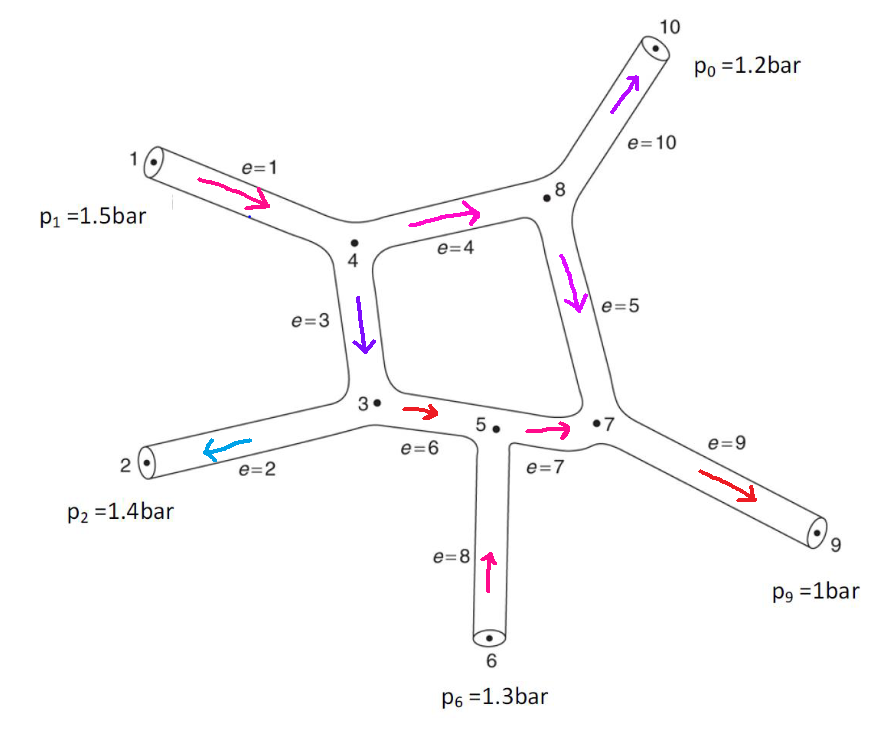
\includegraphics[width=\textwidth]{HW1/PaintResults.png}
    \caption{The piping system diagram with flow directions drawn on, the flow rates are represented with colors, Red being high and blue low.}
    \label{hw1:fig:flows}
\end{figure}

The program could me modified to solve Example 1.6 from Chapter 1 on the book by Rao by changing the boundary conditions and the finite element equation and use instead the spring finite element equation:

$$\left[K^{(e)}\right]=k_e\left[\begin{array}{rr}
1 & -1 \\
-1 & 1 
\end{array}\right] $$

\newpage
\appendix
\section{Code}
\lstinputlisting[caption=The Matlab program used, , language=Matlab]{HW1/A1.m}



\end{document}
